We decided to have time tracking data stored in Git Notes for every repo so that it can be tightly tied to code.
This gives us opportunity to have more complete overview when and on what issue / branch the time was spent.
It also gives access to a features such as git diff that can be used for measuring writing speed.
Furthermore, it lifts a job from our shoulders by handling complex cases such as rebase and merge for us.

The downside is that git notes take up some space on client machine and Git server.
They can also be externally edited, and they might cause issues with git usage if developer does not follow best practices.
Nonetheless, we decided to go this way as the space used by git notes is fractional compared to file sizes, and our app is a tool for the developer,
so we don't see any urgent need to protect it from him.

We also found open source CLI app made for local time-tracking with Git, so we decided to base our app on the already existing code and add more functionality.
There is always an option to switch to external database for storing this kind of data but there is no reason to so at the moment.

Partly enforced by the usage of git, the general design is shown on Figure TODO.
\begin{figure}[h]
    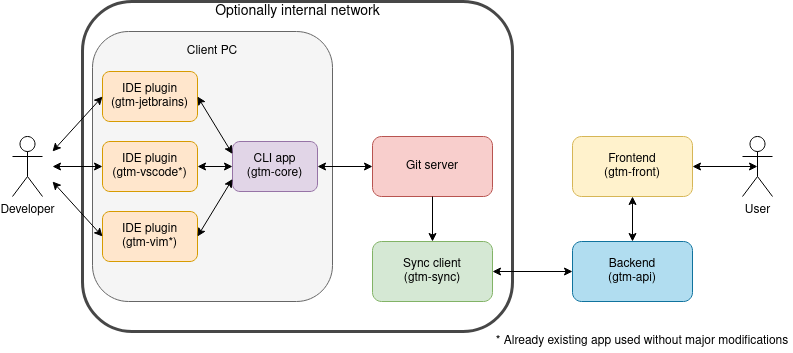
\includegraphics[width=\textwidth]{figures/project_archidecture}\label{fig:project-archidecture}
\end{figure}

The general time-tracking application can be divided into three different kind of smaller applications:
\begin{enumerate}
    \item \textbf{Applications that are responsible for data collecting.} These applications are CLI app and IDE plugins and are installed on developers machine.
    \item \textbf{Applications that are responsible for syncing data.} This role is filled by a Sync client, and these applications are installed onto companies servers where they can access git internal network.
    \item \textbf{Applications that are responsible for analyzing and displaying data.} These are Frontend and Backend app that can be installed on any public server.
\end{enumerate}

The reasoning behind this architecture is scalability and security.
For every Backend there can be multiple Sync clients all installed on different machines and with different Git access rights.
For every Sync client there can be multiple Client apps all logging time independent of one another.
And in the end, there can be multiple IDE plugins interacting with CLI app.

For security, it is very important to ensure, that no sensitive information is leaked.
To deal with this issue many companies have their Git available only in an internal network.
Not to rise any more security concerns we decided to follow the same principle and not export any git code outside internal network.
That is the reason, why Sync client is needed as it has access to internal network, but only uploads time-tracking related information to our Backend.
Therefore, actual code never leaves an internal network.

All the applications that are installed on either client machine or client server are open source so that the client can easily verify,
they only do what they are meant to do.

\section{Client CLI app}\label{sec:cli-app}
%TODO(Tavo): ...

\section{IDE plugins}\label{sec:ide-plugins}
%TODO(Tavo): ...

\section{Sync client}\label{sec:sync-client}
%TODO(Tavo): ...

\section{Backend}\label{sec:backend}
%TODO(Marten): ...

\section{Frontend}\label{sec:frontend}
%TODO(Marten): ...